\documentclass[11pt]{exam}		%Doc : https://mirrors.ircam.fr/pub/CTAN/macros/latex/contrib/exam/examdoc.pdf

% \printanswers					%Comment this line to hide the answers 

\pointpoints{point}{points}
\addpoints

%%%%%%%%%%%%%%%%%%%%%%%%%%%%%%%%%%%%%%%%%
% Cleese Assignment
% Structure Specification File
% Version 1.0 (27/5/2018)
%
% This template originates from:
% http://www.LaTeXTemplates.com
%
% Author:
% Vel (vel@LaTeXTemplates.com)
%
% License:
% CC BY-NC-SA 3.0 (http://creativecommons.org/licenses/by-nc-sa/3.0/)
% 
%%%%%%%%%%%%%%%%%%%%%%%%%%%%%%%%%%%%%%%%%

%----------------------------------------------------------------------------------------
%	PACKAGES AND OTHER DOCUMENT CONFIGURATIONS
%----------------------------------------------------------------------------------------

\usepackage{lastpage} % Required to determine the last page number for the footer

\usepackage{graphicx} % Required to insert images

\setlength\parindent{0pt} % Removes all indentation from paragraphs

\usepackage[svgnames]{xcolor} % Enabling colors by their 'svgnames'
\usepackage[most]{tcolorbox} % Required for boxes that split across pages

\usepackage{booktabs} % Required for better horizontal rules in tables

\usepackage{listings} % Required for insertion of code

\usepackage{etoolbox} % Required for if statements

\usepackage{multido} % required for dotted lines

\usepackage[french]{babel} % English language hyphenation

\usepackage{svg}

%----------------------------------------------------------------------------------------
%	MARGINS
%----------------------------------------------------------------------------------------

\usepackage{geometry} % Required for adjusting page dimensions and margins

\geometry{
	paper=a4paper, % Change to letterpaper for US letter
	top=3cm, % Top margin
	bottom=3cm, % Bottom margin
	left=2.5cm, % Left margin
	right=2.5cm, % Right margin
	headheight=14pt, % Header height
	footskip=1.4cm, % Space from the bottom margin to the baseline of the footer
	headsep=1.2cm, % Space from the top margin to the baseline of the header
	%showframe, % Uncomment to show how the type block is set on the page
}

%----------------------------------------------------------------------------------------
%	FONT
%----------------------------------------------------------------------------------------
\usepackage{fontspec}
\usepackage{unicode-math}
\usepackage[utf8]{inputenc} % Required for inputting international characters
\usepackage[T1]{fontenc} % Output font encoding for international characters

\setmainfont[Ligatures=TeX]{Caladea}
%----------------------------------------------------------------------------------------
%	HEADERS AND FOOTERS
%----------------------------------------------------------------------------------------

\usepackage{fancyhdr} % Required for customising headers and footers

\pagestyle{fancy} % Enable custom headers and footers

% \lhead{\small\assignmentClass\ifdef{\assignmentClassInstructor}{\ (\assignmentClassInstructor):}{}\ \assignmentTitle} % Left header; output the instructor in brackets if one was set
% \chead{} % Centre header
% \rhead{\small\ifdef{\assignmentAuthorName}{\assignmentAuthorName}{\ifdef{\assignmentDueDate}{Due\ \assignmentDueDate}{}}} % Right header; output the author name if one was set, otherwise the due date if that was set

% \lfoot{} % Left footer
% \cfoot{\small Page\ \thepage\ sur\ \pageref{LastPage}} % Centre footer
% \rfoot{} % Right footer

% \renewcommand\headrulewidth{0.5pt} % Thickness of the header rule


% \fancypagestyle{plain}{
% 	\lhead{} % Left header; output the instructor in brackets if one was set
% 	\chead{} % Centre header
% 	\rhead{}

%   \renewcommand{\headrulewidth}{0pt}%
%   \fancyfoot[C]{\small Page\ \thepage\ sur\ \pageref{LastPage}}%
% }

%----------------------------------------------------------------------------------------
%	MODIFY SECTION STYLES
%----------------------------------------------------------------------------------------

% \usepackage{titlesec} % Required for modifying sections

%------------------------------------------------
% Section

% \titleformat
% {\section} % Section type being modified
% [block] % Shape type, can be: hang, block, display, runin, leftmargin, rightmargin, drop, wrap, frame
% {\Large\bfseries} % Format of the whole section
% {\assignmentQuestionName~\thesection} % Format of the section label
% {6pt} % Space between the title and label
% {} % Code before the label

% \titlespacing{\section}{0pt}{0.5\baselineskip}{0.5\baselineskip} % Spacing around section titles, the order is: left, before and after

%------------------------------------------------
% Subsection

% \titleformat
% {\subsection} % Section type being modified
% [block] % Shape type, can be: hang, block, display, runin, leftmargin, rightmargin, drop, wrap, frame
% {\itshape} % Format of the whole section
% {(\alph{subsection})} % Format of the section label
% {4pt} % Space between the title and label
% {} % Code before the label

% \titlespacing{\subsection}{0pt}{0.5\baselineskip}{0.5\baselineskip} % Spacing around section titles, the order is: left, before and after

% \renewcommand\thesubsection{(\alph{subsection})}

%----------------------------------------------------------------------------------------
%	CUSTOM QUESTION COMMANDS/ENVIRONMENTS
%----------------------------------------------------------------------------------------


%	TITLE SECTION
%----------------------------------------------------------------------------------------

% \newcommand{\authorstyle}[1]{{\large\usefont{OT1}{phv}{b}{n}#1}} % Authors style (Helvetica)

% \newcommand{\institution}[1]{{\footnotesize\usefont{OT1}{phv}{m}{sl}#1}} % Institutions style (Helvetica)

% \usepackage{titling} % Allows custom title configuration

% \newcommand{\HorRule}{\rule{\linewidth}{1pt}} % Defines the gold horizontal rule around the title

% \pretitle{
% 	\centering
% 	\vspace{-120pt} % Move the entire title section up
% 	\HorRule\vspace{10pt} % Horizontal rule before the title
% 	% \textbf
% 	\bfseries
% 	\fontsize{32}{36}
% 	\usefont{T1}{phv}{b}{n}
% 	\selectfont % Helvetica
% 	\color{DarkRed} % Text colour for the title and author(s)
% }

% \posttitle{\par\vskip 15pt} % Whitespace under the title

% \preauthor{} % Anything that will appear before \author is printed

% \postauthor{ % Anything that will appear after \author is printed
% 	% \vspace{10pt} % Space before the rule
% 	\par\HorRule % Horizontal rule after the title
% 	\vspace{-30pt} % Space after the title section
% }


\usepackage{blindtext, subfig}
\usepackage{dblfloatfix} % fix for bottom-placement of figure
\usepackage{wrapfig}

%----------------------------------------------------------------------------------------
%	REQUIRED
%----------------------------------------------------------------------------------------
\newcommand{\Titre}{Électricité} % 
\newcommand{\ConsignesGenerales}{
	
	\begin{itemize}
		\item Noter nom et prénom et classe en haut à gauche de la page.
		\item Répondre aux questions sur les pointillés.
		\item Répondre aux questions par des phrases.
		\item Essayer de répondre à toutes les questions.
		\item Ne pas perdre trop de temps si on ne sait pas/comprends 
		pas et passer à la suite pour avoir un maximum de points! 
		% \item Ne pas se décourager :)
		\vspace{-5pt}
	\end{itemize}}

\title{\Titre}
\begin{document}
\thispagestyle{headandfoot}

\section{\Titre} % peut faire une partie d'un gros examen

\headrule
\footrule
\setlength{\columnsep}{0.25cm}
\setlength{\columnseprule}{1pt}



\begin{center}
	\begin{tcolorbox}[
		title=Consignes,
		sidebyside,
		colback=red!5!white,
		colframe=red!75!black,
		colbacktitle=yellow!30!red!50!white,
		coltitle=red!25!black,
		fonttitle=\bfseries,
		subtitle style={boxrule=0.4pt,
		colback=yellow!50!red!25!white} ]
		\ConsignesGenerales

		\tcblower

		% \tcbincludegraphics[width=0.2\columnwidth]{logo.png}
		\tcbincludegraphics[height=3.5cm, size=tight, colframe=red, boxrule=1pt, arc=10pt, auto outer arc, clip upper]{logo.png}
		
		% \tcbsubtitle{Second subtitle}
		% Further text.
		\end{tcolorbox}
\end{center}

%----------------------------------------------------------------------------------------
%	EDIT QUESTIONS HERE
%----------------------------------------------------------------------------------------
{\huge Partie cours}

\begin{questions}
	\question[2] 
	\textbf{Écrire le nom} de deux matériaux conducteurs.
	\answerbox{1}{Le fer et l'aluminium sont conducteurs.}
	
	\question[2] 
	\textbf{Écrire le nom} de deux matériaux isolants.
	\answerbox{1}{Le bois et le verre sont isolants.}
	
	\question[2] 
	\textbf{Écrire le nom} de quatre dipôle.
	\answerbox{1}{La pile, la lampe, la diode et le moteur sont des dipôles.}
	
	\question[2] 
	\textbf{Expliquer} ce qui fait qu'un matériau est conducteur ou isolant.
	\answerbox{2}{Un matériaux est conducteur si il laisse passer l'électricité.}
	
	\question[4] 
	\textbf{compléter} le tableau suivant avec les symboles normalisés 
	ou le nom des dipôles correspondant.
    \vspace{20pt}
	% \setlength{\arrayrulewidth}{0.5mm}
	% \setlength{	abcolsep}{18pt}
	%\renewcommand{\arraystretch}{1.5}
	\begin{center}
		% \hspace{-70pt}
	\begin{tabular}{|c|p{4cm}|||||c|p{4cm}|}
		\hline
		Dipôles & symboles normalisé & Dipôles & symboles normalisé \\
		\hline
		interrupteur ouvert & \vspace{25pt} & diode  & \\
		\hline
		DEL (diode electro luminescente) & \vspace{25pt} & resistance  & \\
		\hline
		%générateur 
		& \hspace*{-1cm}\begin{minipage}{.3\textwidth}
			\begin{center}
				\vspace{0.5cm}
				
\includegraphics[width=2.5cm]{generator.png}
			\end{center}
		  \end{minipage} 
		& %pile
		& \hspace*{-1cm}\begin{minipage}{.3\textwidth}
			\begin{center}
				\vspace{0.5cm}
				
\includegraphics[width=2.5cm]{pile.png}
			\end{center}
		  \end{minipage}
		\\
		& 
		&  
		&  \\ \hline
		%moteur 
		& \hspace*{-1cm}\begin{minipage}{.3\textwidth}
			\begin{center}
				% \vspace{0.5cm}
				
\includegraphics[width=2.5cm]{motor.png}
			\end{center}
		  \end{minipage}  
		& %lampe  
		& \hspace*{-1cm}\begin{minipage}{.3\textwidth}
			\begin{center}
				% \vspace{0.5cm}
				
\includegraphics[width=2.5cm]{lampe.png}
			\end{center}
		  \end{minipage} \\
		\hline
		\end{tabular}
	\end{center}
	
	\vspace{10cm}

	{\huge Partie application}
	\question[8] 
	En dessous de chaque circuit, \textbf{dessiner} son \underline{schéma normalisé} à la règle et au crayon à papier.
	\begin{figure*}[hb]
		\centering		
		\subfloat[][]{
		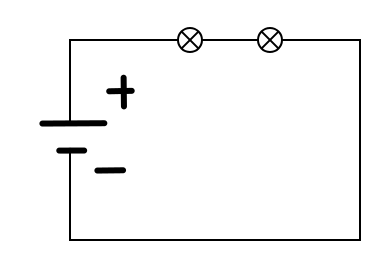
\includegraphics[width=0.35\columnwidth]{circuit1.png}
		}
		\hspace{5cm}
		\subfloat[][]{
		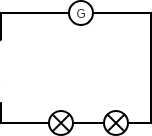
\includegraphics[width=0.35\columnwidth]{circuit2.png}
		}
	% \end{figure*}
	\vspace{6cm}
	% \begin{figure*}[hb]
		\centering		
		\subfloat[][]{
		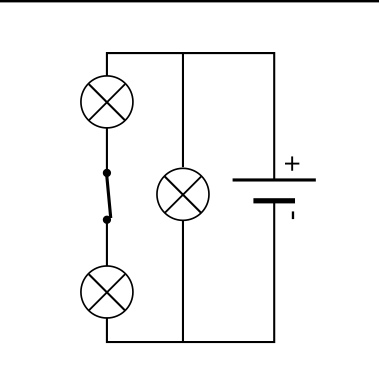
\includegraphics[width=0.35\columnwidth]{circuit3.png}
		}
		\hspace{5cm}
		\subfloat[][]{
		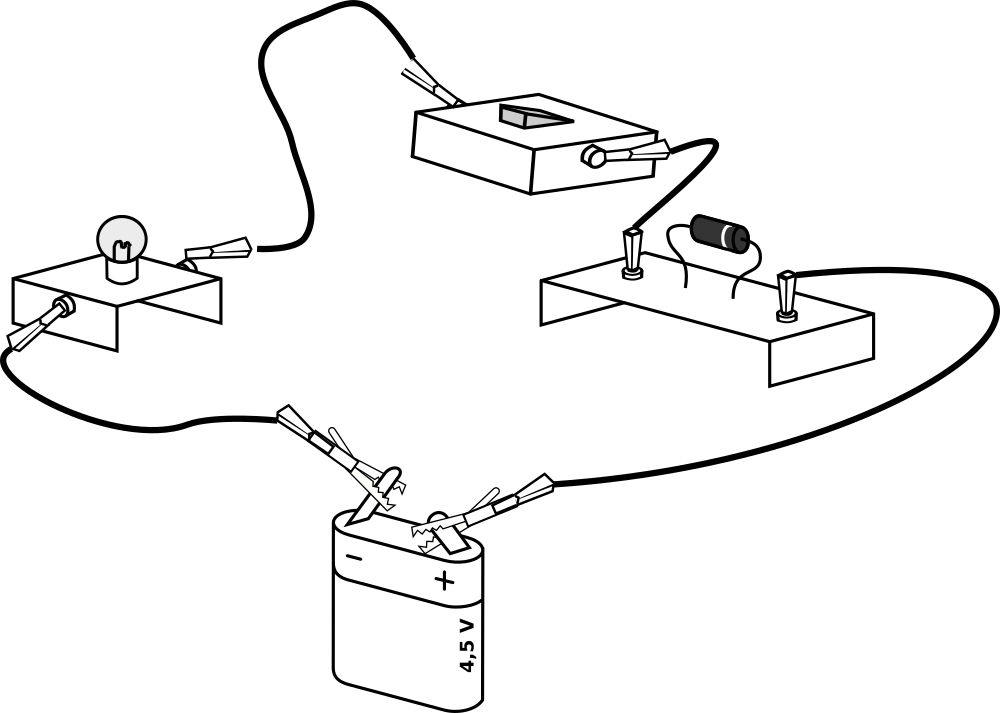
\includegraphics[width=0.35\columnwidth]{circuit4.png}
		}
	\end{figure*}


\end{questions}

\vfill
\begin{center}
\setlength{\doublerulesep}{0.25in}
\multirowgradetable{1}[questions]
\vspace{-25pt}
\end{center}


\end{document}